\documentclass{article}
\usepackage{enumerate}
\usepackage{amsmath}
\usepackage{amssymb}
\usepackage{graphicx}
\usepackage{subfigure}
\usepackage{geometry}
\usepackage{caption}
\usepackage{indentfirst}
\usepackage{fancyhdr}
\usepackage{ulem}
\usepackage{multirow}
\usepackage{tabu}
\usepackage{array}

\title{MA209 Homework 1}
\author{Liu Yihao 515370910207}
\date{}
\pagestyle{fancy}
\fancyhead{}
\fancyhead[C]{
\includegraphics[width=\linewidth]{ji_header.png}}
\fancyfoot[C]{\thepage}
\renewcommand{\headrulewidth}{0pt}
\addtolength{\headheight}{4\baselineskip}
\geometry{top=4cm,bottom=4.0cm}
\begin{document}

\vspace*{3mm}

\begin{minipage}{0.6\linewidth}
\ 
\end{minipage}
\hfill
\begin{minipage}{0.38\linewidth}
\begin{center}
\huge\bfseries
Lab Report \\[8mm]
\fontsize{100pt}{\baselineskip}\selectfont
2
\end{center}
\end{minipage}

\vspace*{1cm}

{\huge\bfseries
\uline{UM-SJTU Joint Institute \phantom{xxxxxxxxxxxx}}
\vspace*{2mm}

Ve270 Introduction to Logic Design
}	

\vspace*{2cm}
\begin{center}
\LARGE
by \\[2mm]
\begin{tabular}{ll}
Liu Yihao & 515370910207 \\
Ma ShiYao & 515370910157
\end{tabular}

\vspace*{2cm}
Date: 2017-06-06
\end{center}

\vspace*{2cm}
\begin{center}
\Huge\bfseries
Design of an SSD Driver
\end{center}

\newpage

\section{Objectives}
To design a Seven-Segment Display (SSD) driver using Xilinx ISE, and to implement the circuit in an FPGA chip.

\section{Problem Definition}
To form SSD as a digit-display system. By inputting 4-bit binary number, seven cathode will receive a 7-bit binary digit for the seven segments of the LED, then the corresponding parts of the LED will illuminate to form the correct decimal digit. When the cathode receives a ``0'' and the anode receives an ``1"", the LED is turned on. The input of this system is a 4-bit binary number, the output is the corresponding decimal digit displayed by LED. As an example, when the driver receives ``0101"" as input, the decimal number ``5"" will be displayed.

\section{System Partitioning}
\begin{enumerate}
\item Switch and driver: switches and driver are used to input 4-bit binary digit signal. By toggling different switches, the driver will receive the binary digit inputted, then convert it to anodes and cathodes.
\item Anodes and cathodes: used for receiving the signal from driver, and controlling the LED segments.
\item LED segments: to receive the signal converted fro the anodes and cathodes, and illuminate to form the corresponding decimal digit.
\end{enumerate}

\section{Design Entry}
The overall truth table was shown in Table \ref{truth-table}.

\begin{table}[!hbtp]
\centering
\begin{tabular}{|p{1cm}<{\centering}|p{1cm}<{\centering}|p{1cm}<{\centering}|p{1cm}<{\centering}|p{1cm}<{\centering}|p{1cm}<{\centering}|p{1cm}<{\centering}|p{1cm}<{\centering}|}
\hline
\multirow{2}{*}{Input} & \multicolumn{7}{c|}{ Outputs(LED segments) }\\\cline{2-8}
& CA & CB & CC & CD & CE & CF & CG \\\hline
0001 & 0 & 1 & 1 & 0 & 0 & 0 & 0 \\\hline
0010 & 1 & 1 & 0 & 1 & 1 & 0 & 1 \\\hline
0011 & 1 & 1 & 1 & 1 & 0 & 0 & 1 \\\hline
0100 & 0 & 1 & 1 & 0 & 0 & 1 & 1 \\\hline
0101 & 1 & 0 & 1 & 1 & 0 & 1 & 1 \\\hline
0110 & 1 & 0 & 1 & 1 & 1 & 1 & 1 \\\hline
0111 & 1 & 1 & 1 & 0 & 0 & 0 & 0 \\\hline
1000 & 1 & 1 & 1 & 1 & 1 & 1 & 1 \\\hline
1001 & 1 & 1 & 1 & 1 & 0 & 1 & 1 \\\hline
\end{tabular}
\caption{Overall truth table}
\label{truth-table}
\end{table}

First, we designed some macros to translate different inputs into numbers, for example, the schematics design and symbol for input number 1 (0001) was shown in Figure \ref{design-digit-1}.\\

\begin{figure}[!hbtp]
\centering
\subfigure[Schematics design]{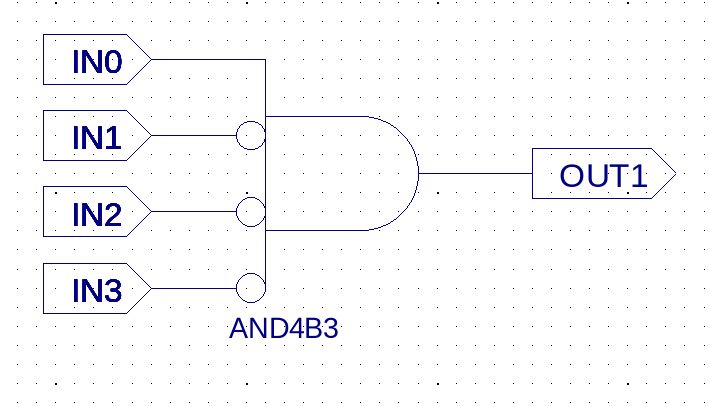
\includegraphics[width=0.4\linewidth]{digit1_sch.png}}
\subfigure[Symbol]{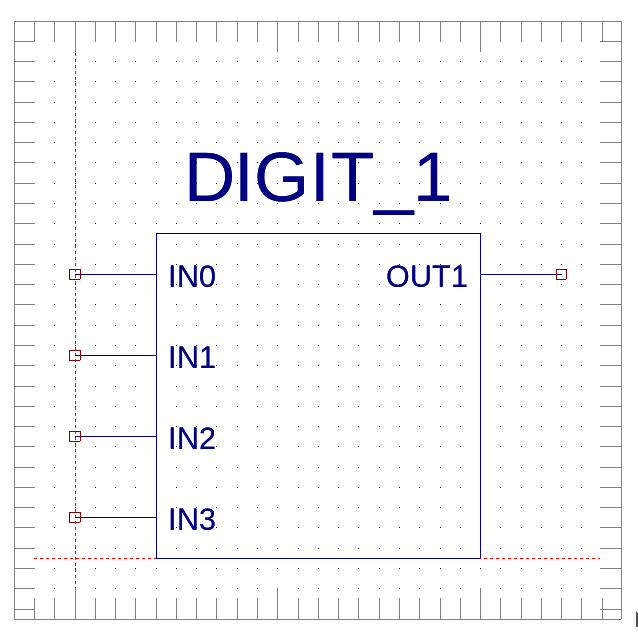
\includegraphics[width=0.25\linewidth]{digit1_sym.png}}
\caption{Schematics design and symbol for input number 1}
\label{design-digit-1}
\end{figure}

According to this truth table, we designed a circuit for each input segment, shown in Figure \ref{design-segment}. \\

\begin{figure}[!hbtp]
\centering
\subfigure[CA]{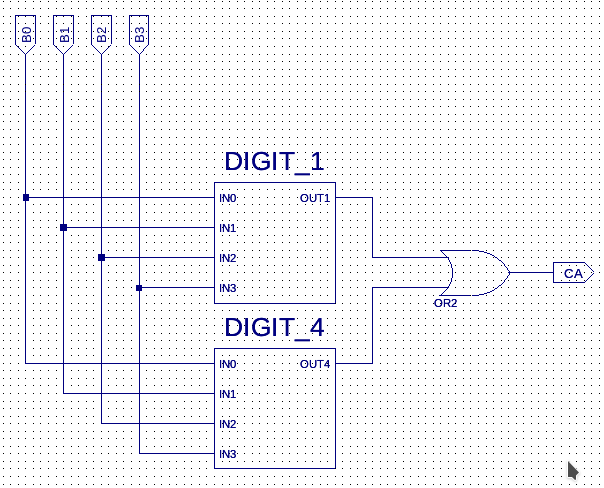
\includegraphics[width=0.3\linewidth]{ca.png}}
\subfigure[CB]{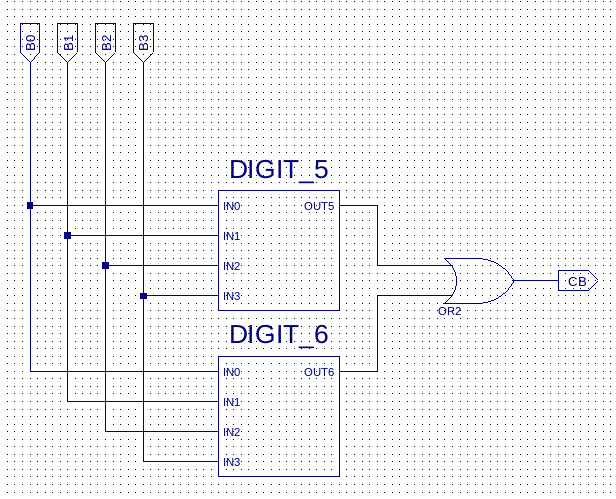
\includegraphics[width=0.3\linewidth]{cb.png}}
\subfigure[CC]{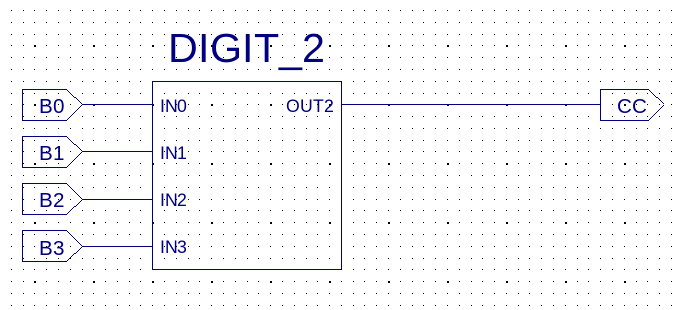
\includegraphics[width=0.3\linewidth]{cc.png}}
\subfigure[CD]{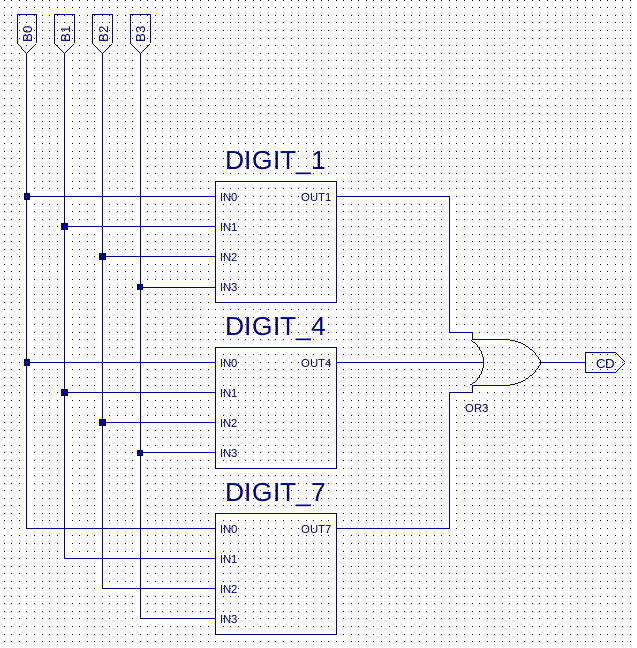
\includegraphics[width=0.3\linewidth]{cd.png}}
\subfigure[CE]{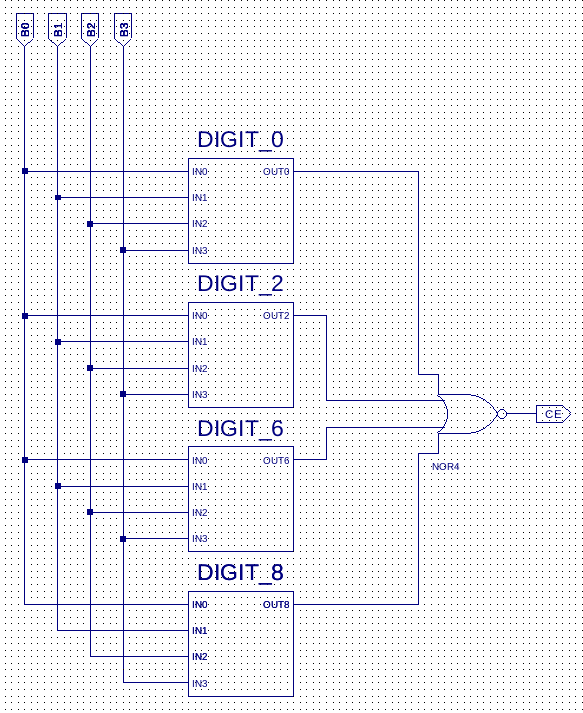
\includegraphics[width=0.3\linewidth]{ce.png}}
\subfigure[CF]{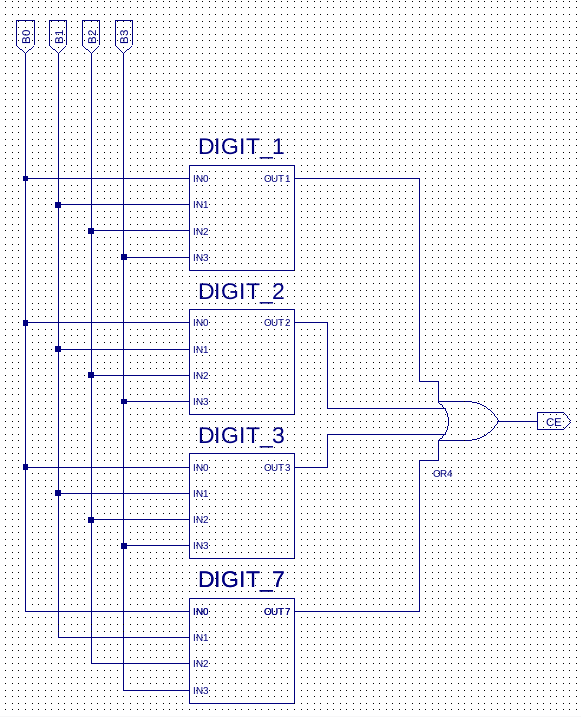
\includegraphics[width=0.3\linewidth]{cf.png}}
\subfigure[CG]{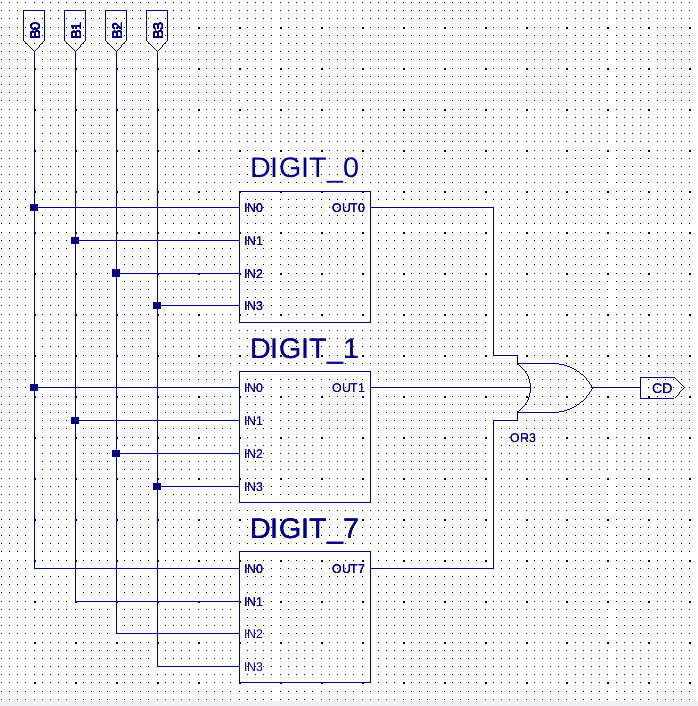
\includegraphics[width=0.3\linewidth]{cg.png}}
\caption{Schematics design for input segments}
\label{design-segment}
\end{figure}

At last, we build the symbols for the seven input segments and designed a final circuit of SSD, shown in Figure \ref{design-ssd}. \\

\begin{figure}[!hbtp]
\centering
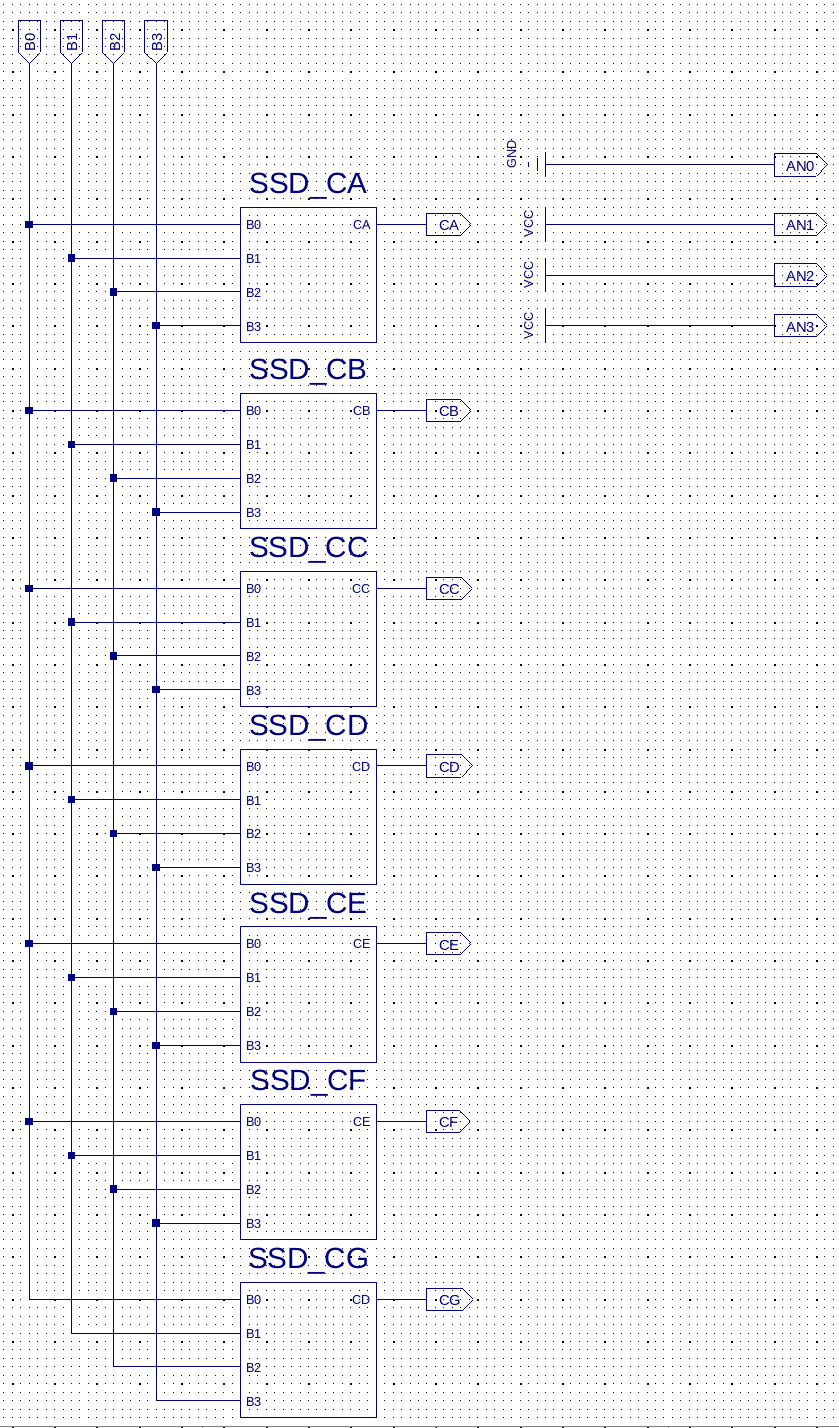
\includegraphics[width=0.7\linewidth]{ssd.png}
\caption{Schematics design for SSD}
\label{design-ssd}
\end{figure}

\newpage

\section{Test Plan}
\begin{center}
\begin{tabular}{|m{3cm}<{\centering}|m{10cm}|}
\hline
Test content & \multicolumn{1}{c|}{Test method} \\\hline
CA & \multirow{7}{10cm}{Input signal that needs corresponding LED segment to illuminate, then observe if it illuminates. If it illuminates when corresponding signal inputted, this subsystem passes the test; otherwise it fails.} \\\cline{1-1}
CB & \\\cline{1-1}
CC & \\\cline{1-1}
CD & \\\cline{1-1}
CE & \\\cline{1-1}
CF & \\\cline{1-1}
CG & \\\hline
The overall system & Input every kind of the 4-bit binary digit signal: 0001, 0010, 0011, 0100, 0101, 0110, 0111, 1000, 1001, then observe if LED displays the corresponding decimal digit:1,2,3,4,5,6,7,8,9. If so, the system passes the test; otherwise it fails. \\\hline
\end{tabular}
\end{center}

\section{Simulation Results}
We simulated the result of the overall system with input values B0,B1,B2,B3 as 0001, 0010, 0011, 0100, 0101, 0110, 0111, 1000, 1001. The result was shown in Figure \ref{simulation}.

\begin{figure}[!hbtp]
\centering
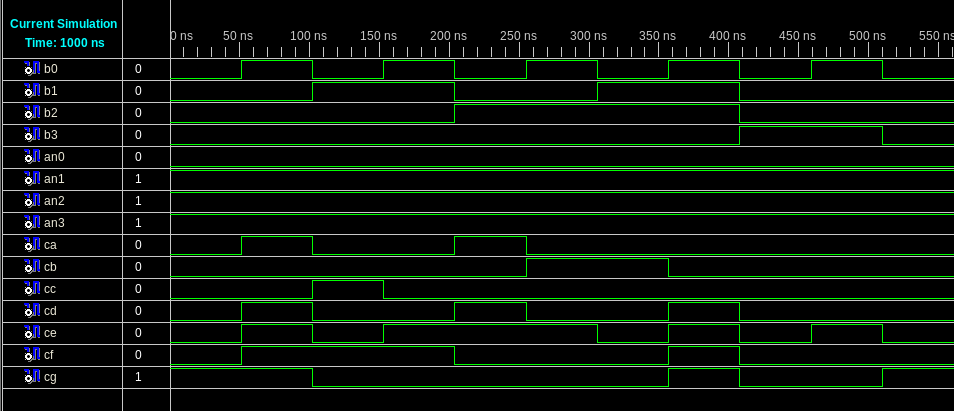
\includegraphics[width=0.9\linewidth]{simulation.png}
\caption{Simulation of SSD}
\label{design-ssd}
\end{figure}

We found the values in the simulation identical to the truth table we built as Table \ref{truth-table}, which proved that our design was right.

\newpage

\section{Conclusion}


\section{Appendix}
The schematics of our design, as well as the \TeX\ source code, were attached to the report.


\end{document}